\chapter{Laser Drilling}

Laser drilling is ablation on a single spot.  \textbf{Ablation} is removal of material from the surface of an 
object by vaporization, chipping or other erosive process. 

\textbf{Laser ablation} is ablation by using a laser. Typically, we use pulsed lasers. The most important property of the
beam is laser intensity. 

One type of material removal is melt overflow:
\begin{itemize}
    \item Absorption \pd  Laser beam is absorbed in the  surface and transformed  into heat.
    \item Fusion \pd $I \ge 10^5 \frac{W}{cm^2}$, Melt pool is formed when the melting temperature is reached.
    \item Evaporation \pd $I \ge 10^6 \frac{W}{cm^2}$, Above the melting temperature material vapour expands. 
\end{itemize}
Shown on figure \ref{fig:ldm}.
\begin{figure}[h!]
    \centering
    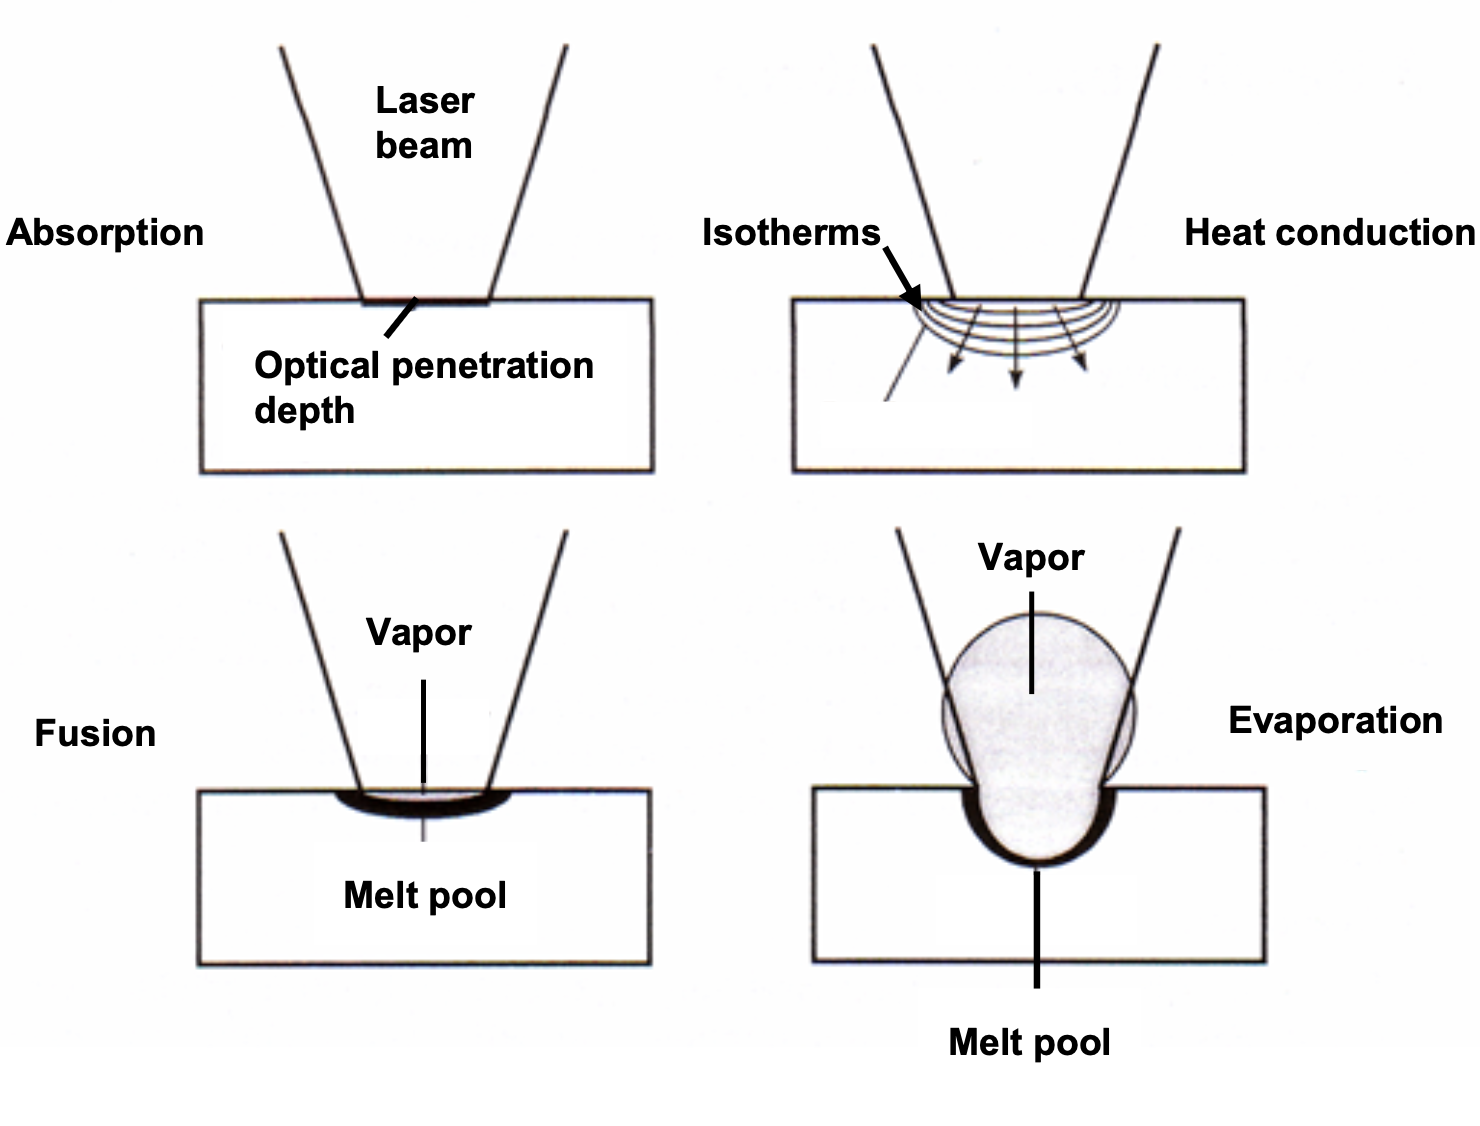
\includegraphics[width=0.4\textwidth]{slike/ldm.png}
    \caption{Beam-matter interaction for drilling}
    \label{fig:ldm}
\end{figure}
Ablation happens primarily by the \textbf{melt overflow} or \textbf{sublimation}.
Figure \ref{fig:melt} show the process schematics of laser material ablation.
\begin{figure}[h!]
    \centering
    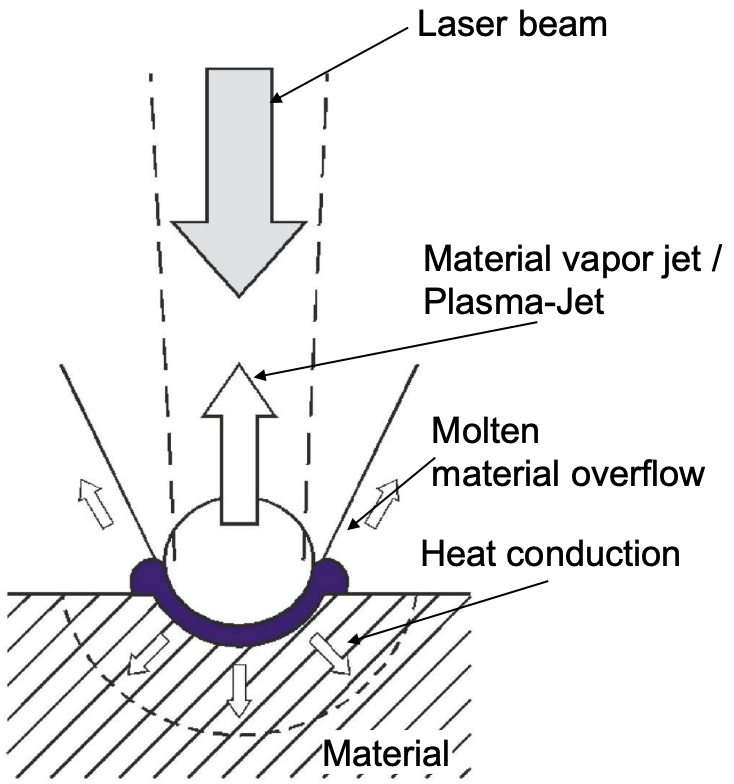
\includegraphics[width=0.25\textwidth]{slike/meltflow.png}
    \caption{Schematics of the melt flow. \sln}
    \label{fig:melt}
\end{figure}

Pulse width influences both \textit{efficiency} and \textit{precision}. Shown on figure \ref{fig:ldep}.
\begin{figure}[h!]
    \centering
    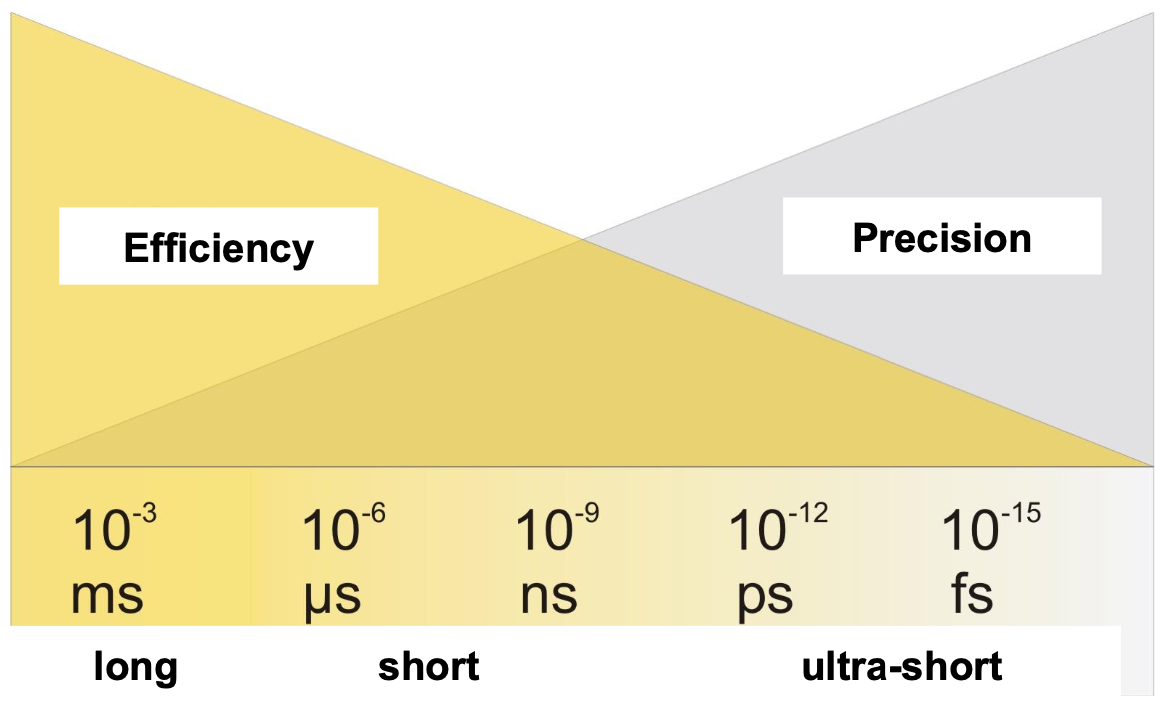
\includegraphics[width=0.4\textwidth]{slike/ldep.png}
    \caption{Efficiency and Precision. \sln}
    \label{fig:ldep}
\end{figure}

\section{Laser ablation with short and Ultra-short pulses}
With short pulses the ablation process is:\newline
Absorption \pd Heating \pd Melting \pd Evaporation \pd Melt overflow

For ultra-short pulses the process is:\newline
Absorption of laser energy by free and bound electrons \pd Energy transfer into the lattice and breaking of intermolecular bonds 
\pd Fast plasma expansion


Figure \ref{fig:uspablation} show the ablation of ultra-short pulses. Note that only the part of materials where
the laser intensity if higher that the \textit{ablation threshold}.

\begin{figure}[h!]
    \centering
    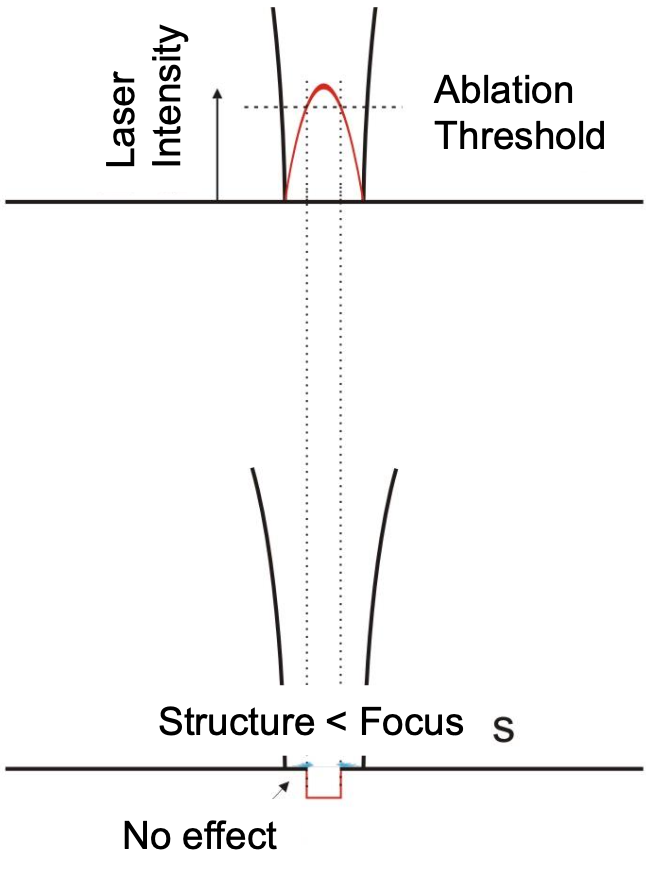
\includegraphics[width=0.25\textwidth]{slike/ablthr.png}
    \caption{USP ablation threshold. \sln}
    \label{fig:uspablation}
\end{figure}

Ablation occurs only if material has received enough energy to get removed. 
How much energy the material has received in a pulse is defined by the \textbf{fluence} F.
Fluence is defined by \ref{eq:F}. Unit is $\frac{J}{m^2}$.
\begin{equation}
    F = \frac{1}{A} \int_{-\infty}^{\infty} P_{pulse}(t) dt \rightarrow I \cdot t
    \label{eq:F}
\end{equation}

Below a certain fluence, material remains unmodified - absorbed energy is dissipated as heat. 

For materials with a \textit{well-defined} ablation threshold, created structure size (crater) is determined by the 
equation \ref{eq:crater}.
\begin{equation}
    d = d_0 \sqrt{ln(\frac{F}{F_{th}})}
    \label{eq:crater}
\end{equation}
Where $d_0$ is the laser beam diameter, $F$ is the laser fluence an $F_{th}$ is the material dependent 
threshold. By changing the fluence, we can control the structure size and achieve sub-wavelength dimensions.

\subsection{Limiting effects}
For ablation, the laser fluence must be bigger than the ablation threshold. 
Tilted surfaces reduce laser intensity, according to $I = \frac{P}{A_0} = \frac{P}{A_0 cos(\alpha)}$.
Absorption stops when surface tilt causes intensity to drop below the threshold. Figure \ref{fig:atilted}
show the effect. This effect causes \textbf{tampered drill holes} and \textbf{Limited drilling depth}.


\begin{figure}[h!]
    \centering
    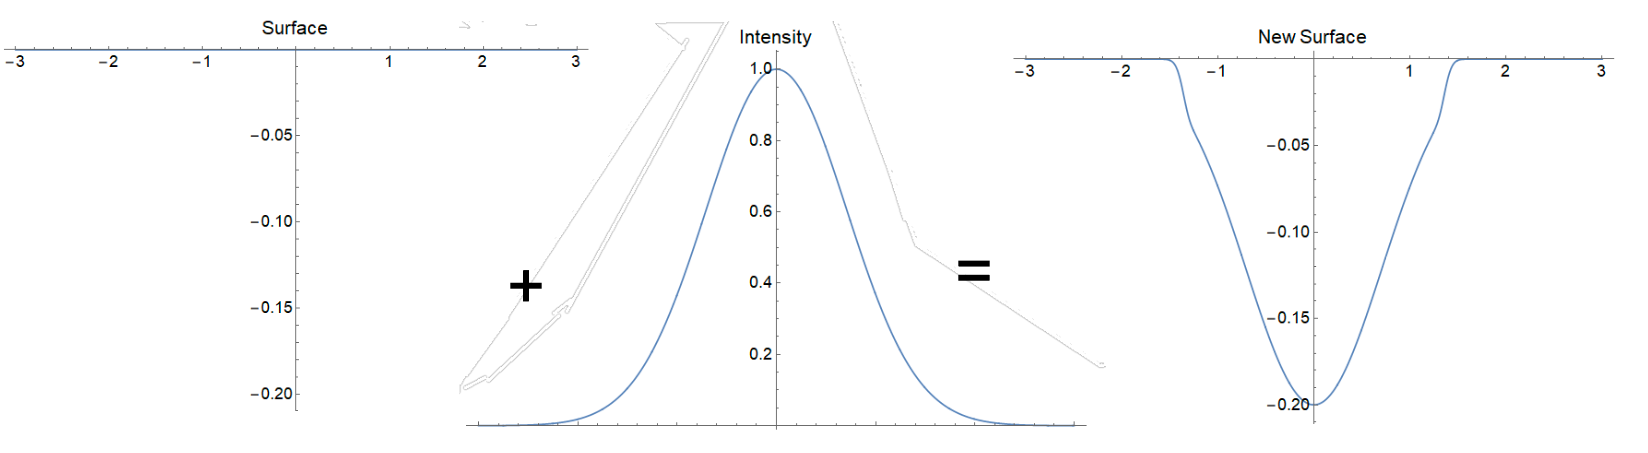
\includegraphics[width=0.5\textwidth]{slike/atillt.png}
    \caption{Effect of tilt.\sln}
    \label{fig:atilted}
\end{figure}

\subsection{Overcoming limitations (of drilling)}

Laser beam can be tilted to compensate for the taper, shown on figure \ref{fig:tiltlim}.
\begin{figure}[h!]
    \centering
    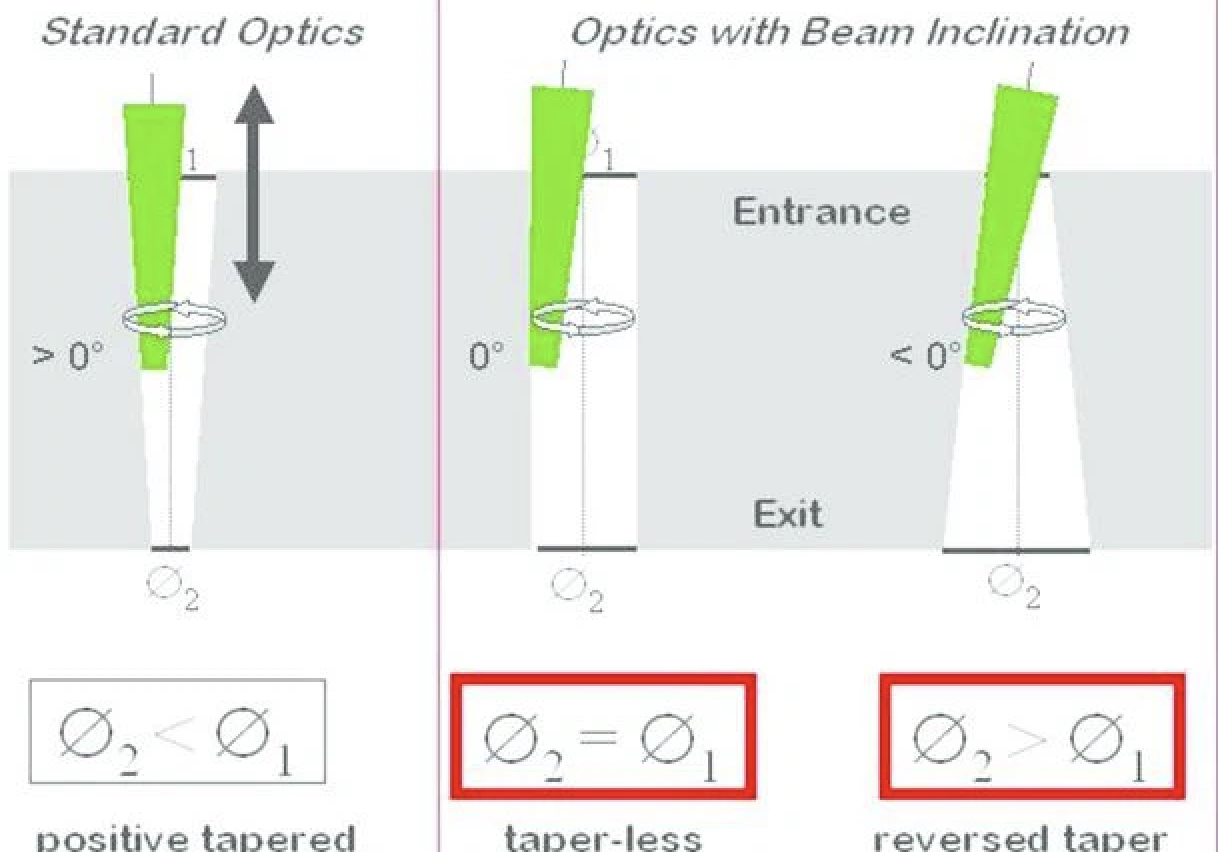
\includegraphics[width=0.5\textwidth]{slike/taper.png}
    \caption{Tilting optics to resolve tilt.\sln}
    \label{fig:tiltlim}
\end{figure}

\section{Specialized technologies}
\subsection{Single and Multi pulse}
Single and multi-pulse (percussion) drilling are very similar, by using multiple pulses the drilling depth can be increased. 
If the needed ablation fluence can't be reached we need to cut a circle \pd helical drilling or trepanning.


\subsection{Helical drilling and Trepanning}
Helical drilling and trepanning are very similar processes, shown on figure \ref{fig:held}.
\begin{figure}[h!]
    \centering
    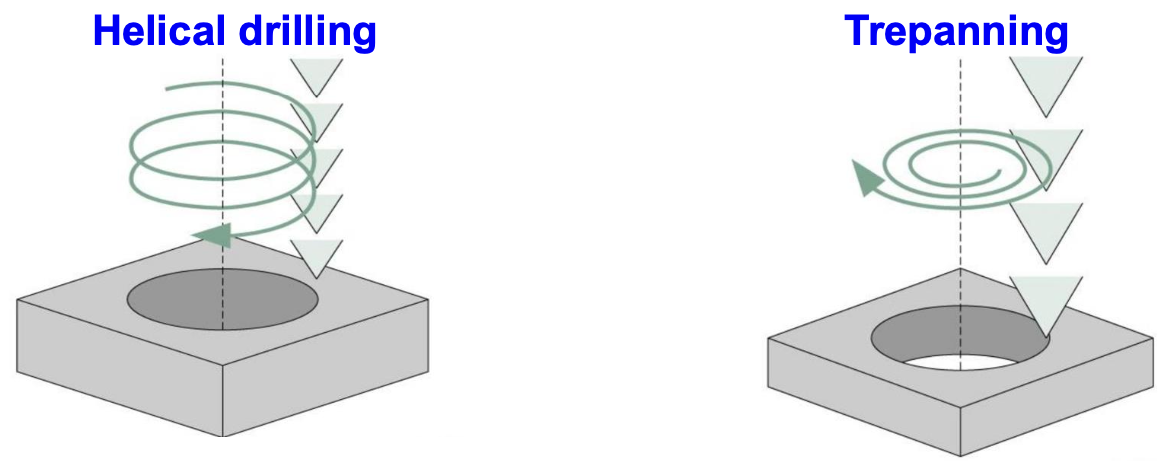
\includegraphics[width=0.5\textwidth]{slike/helical.png}
    \caption{Helical drilling and Trepanning. \sln}
    \label{fig:held}
\end{figure}

Trepanning consists of combined percussion drilling in the middle and then cutting the sample in circular or spiral motion.
Helical drilling is a combination of percussion drilling and circular motion. Both processes are very similar.

\section{Drilling dimensions}
Table \ref{tab:ddims} shows typical values for metals processed with $Nd:YAG$ laser. 

\begin{table}[h!]
    \begin{tabular}{|c|c|c|c|}
        \hline
                            & Single pulse      & Percussion &              Trepanning \\
        \hline
        Typical diameter    & $20\dots 250 \mu m$ & $0,1 \dots 0,5 mm $&$ 0,5 \dots 5 mm$ \\
        \hline
        Maximum drilling depth & $3 mm$ & $ 30 mm$ & $15 mm$ \\
        \hline
    \end{tabular}
    \caption{}
    \label{tab:ddims}
\end{table}

\subsection{Helical drilling with beam inclination}
To shape holes, laser beam can be inclined using optics, as shown on figure \ref{fig:inclin}. 

\begin{figure}[h!]
    \centering
    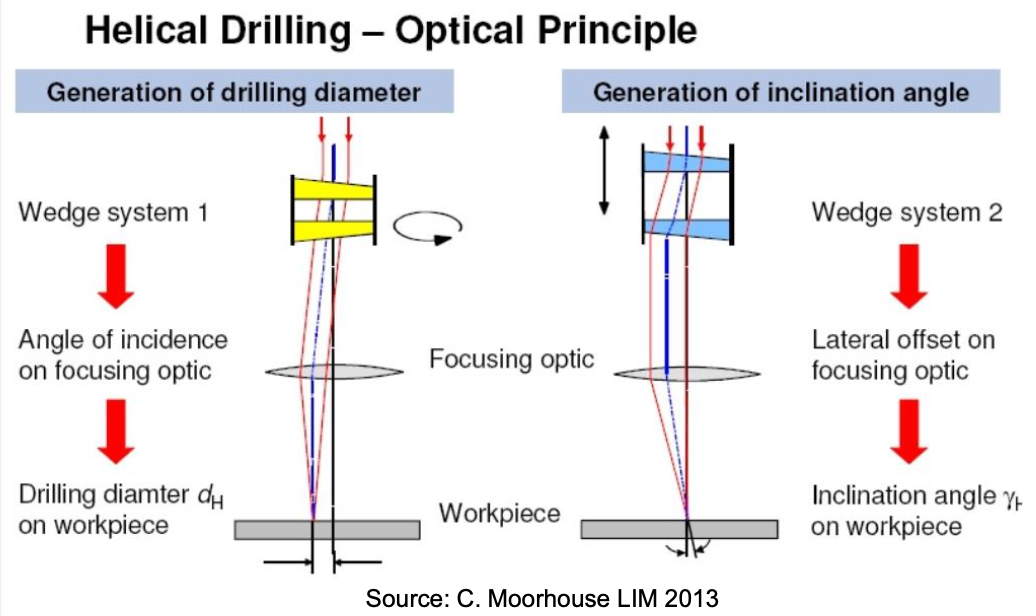
\includegraphics[width=0.5\textwidth]{slike/oinclination.png}
    \caption{Optical principle of helical drilling. \sln}
    \label{fig:inclin}
\end{figure}

Beam is inclined in order to increase the fluence at the boreholes during the drilling process.